\section{Material Properties \blue{Images need updating}}

\subsection{Stress-Strain Diagram}

A \textbf{stress-strain diagram} is the relationship of normal stress as a function of normal strain. One way to collect these measurement is a \textbf{uniaxial tension test} in which a specimen at a very slow, constant rate (quasi-static). A load $P$ and distance $L$ are measured at frequent intervals.

\vspace{5pt}

\noindent Evaluation of average normal strain, or engineering strain (relative to undeformed length):

\[\varepsilon = \frac{\delta}{L_0} = \frac{L-L_0}{L_0}\]

\noindent Evaluation of average normal stress, or engineering stress (relative to undeformed cross section):

\[\sigma = \frac{P}{A_0}\]

\noindent Note that two stress-strain diagrams for a particular material will be similar, but not identical, e.g. because of imperfections, different composition, rate or loading, or temperature.

\begin{figure*}[!h]
\centering
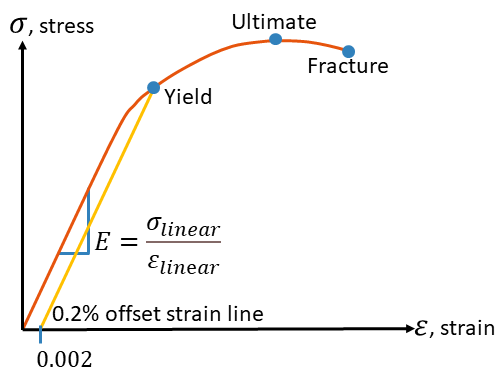
\includegraphics[angle=0, width=3in]{Material Properties-Figures/Stress Strain Diagram.png}
\vspace{-2mm}
\caption{\small Stress-strain diagram showing key properties}
\vspace{-3mm}
\label{Fig:extensometer}
\end{figure*}

\subsubsection{Elastic Behavior}
Loading in this region results \textbf{elastic behavior}, meaning the material returns to its original shape when unloaded. This region of the diagram is mostly a straight line, limited by the proportional limit). This region ends at $\sigma_Y$ (yielding). For $\sigma \le \sigma_{pl}$, the diagram is linear, and the behavior is elastic. For $\sigma_{pl} < \sigma < \sigma_Y$, the diagram is nonlinear, but the behavior is still elastic.

\vspace{3mm}
\noindent \textbf{Young's Modulus}

\vspace{5pt}

\noindent Hooke's law is used for small deformations in the elastic region. The Young's modulus is the slope $E$.
\[\sigma = E\varepsilon\]

\begin{figure*}[!h]
\centering
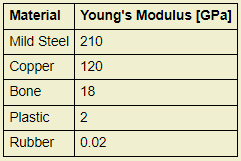
\includegraphics[angle=0, width=2in]{Material Properties-Figures/Modulus Examples.png}
\vspace{-2mm}
\caption{\small Table screenshot from ref pages. Approximate elastic modulus values for different material families.}
\vspace{-3mm}
\label{Fig:ModulusExamples}
\end{figure*}

\vspace{3mm}
\noindent\textbf{Shear Modulus}
\vspace{1mm}
\begin{figure*}[!h]
\centering
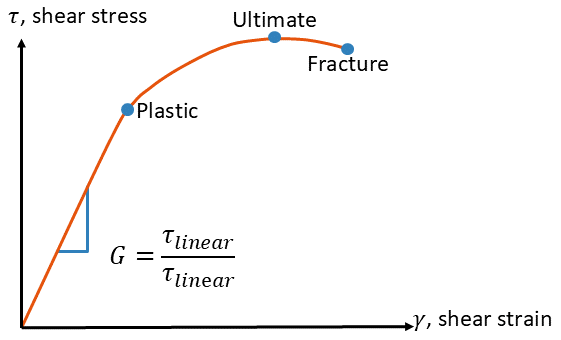
\includegraphics[angle=0, width=4in]{Material Properties-Figures/Shear Diagram.png}
\vspace{-2mm}
\caption{\small \blue{Taken from TAM251 Lecture Notes - L3S14}}
\vspace{-3mm}
\label{Fig:ShearDiagram}
\end{figure*}

\vspace{5pt}
\noindent Hooke's law: \[\tau_{xy} = G\gamma_{xy}\]

\noindent Shear Modulus: \[G = \frac{E}{2(1+\nu)}\]
\noindent Only two of the three material constants (ie; $G$, $E$, $\nu$) are independent in isotropic materials.

\subsubsection{Plastic Behavior}

Stresses above the plastic limit ($\sigma_Y < \sigma$) cause the material to permanently deform.

\vspace{3mm}
\noindent \textbf{Yield Strength}

\vspace{5pt}

\noindent Perfect plastic or ideal plastic: well-defined $\sigma_Y$, stress plateau up to failure. Some materials (e.g. mild steel) have two yield points (stress plateau at $\sigma_{YL}$). Most ductile metals do not have a stress plateau; yield strength $\sigma_{YS}$ is then defined by the \textbf{0.002 (0.2\%) offset method}.

\vspace{3mm}
\noindent \textbf{Strain Hardening}

\begin{figure*}[!h]
\centering
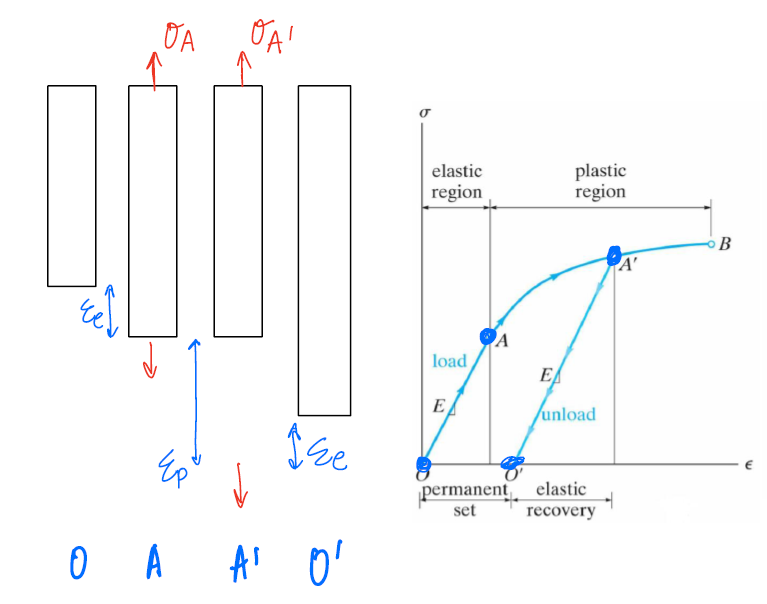
\includegraphics[angle=0, width=4in]{Material Properties-Figures/Strain Hardening.png}
\vspace{-2mm}
\caption{\small \blue{Taken from TAM251 Lecture Notes - L3S8}}
\vspace{-3mm}
\label{Fig:StrainHardening}
\end{figure*}

\noindent \textit{Atoms rearrange} in plastic region of ductile materials when a higher stress is sustained. Plastic strain remains after unloading as \textit{permanent set}, resulting in permanent deformation. Reloading is linear elastic up to the new, higher yield stress (at \textbf{A'}) and a reduced ductility.

\vspace{3mm}
\noindent \textbf{Ultimate Strength}

\vspace{5pt}

\noindent The ultimate strength ($\sigma_u$) is the maximum stress the material can withstand.

\vspace{3mm}
\noindent \textbf{Necking}

\begin{figure*}[!h]
\centering
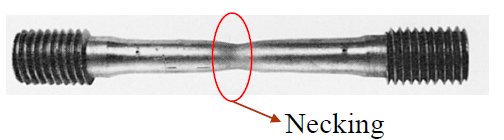
\includegraphics[angle=0, width=3in]{Material Properties-Figures/Necking.png}
\vspace{-2mm}
\caption{\small \blue{Taken from TAM251 Lecture Notes - L3S5}}
\vspace{-3mm}
\label{Fig:Necking}
\end{figure*}

\noindent After ultimate stress ($\sigma_u < \sigma$), the middle of the material elongates before failure.

\vspace{3mm}
\noindent \textbf{Failure}

\vspace{5pt}

\noindent Also called fracture or rupture stress ($\sigma_f$) is the stress at the point of failure for the material. Brittle and Ductile materials fail differently.

\begin{figure*}[!h]
\centering
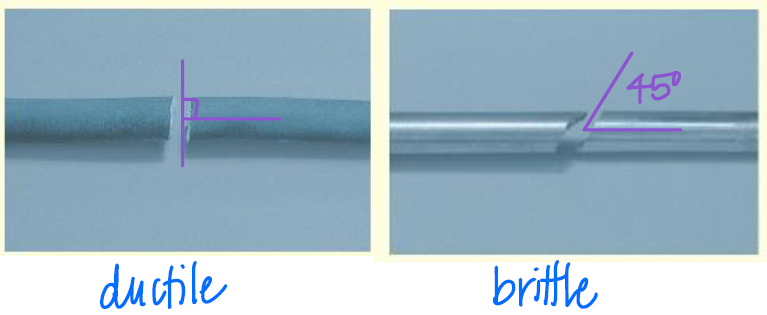
\includegraphics[angle=0, width=3in]{Material Properties-Figures/Ductile vs Brittle.png}
\vspace{-2mm}
\caption{\small \blue{Taken from TAM251 Lecture Notes - L9S19}}
\vspace{-3mm}
\label{Fig:DuctVsBrittle}
\end{figure*}

\begin{itemize}
    \item \textbf{Brittle materials:} small plastic region between yield and failure (fracture), no necking, primary fail by normal stress.
    \item \textbf{Ductile materials:} large region of plastic deformation before failure (fracture) at higher strain, necking; often fails under 45° cone angles by shear stress.
\end{itemize}

\noindent Note the difference between engineering and true stress/strain diagrams: ultimate stress is a consequence of necking, and the true maximum is the true fracture stress.

\vspace{3mm}
\noindent \textbf{Example:} Concrete is a brittle material.

\begin{itemize}
    \item Maximum compressive strength is substantially larger than the maximum tensile strength.
    \item For this reason, concrete is almost always reinforced with steel bars or rods whenever it is designed to support tensile loads.
\end{itemize}

\subsection{Other Derived Properties}

\subsubsection{Directional Materials}
\begin{itemize}
    \item \textbf{Isotropic:} material properties are independent of the direction
    \item \textbf{Anisotropic:} material properties depend on the direction (ie; composites, wood, and tissues)
\end{itemize}

\subsubsection{Poisson's Ratio}
\begin{figure*}[!h]
\centering
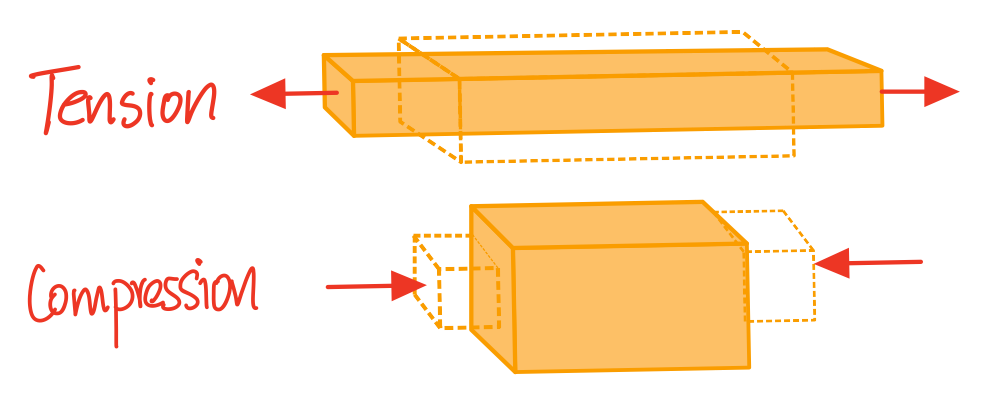
\includegraphics[angle=0, width=4in]{Material Properties-Figures/Poisson's Ratio.png}
\vspace{-2mm}
\caption{\small \blue{Taken from TAM251 Lecture Notes - L3S15}}
\vspace{-3mm}
\label{Fig:PoissonsRatio}
\end{figure*}

\noindent Axial (normal) strain: \[\varepsilon_{x} = \frac{\delta}{L}\]

\noindent Poisson's ratio [$\nu$]: \[\nu = -\frac{lateral strain}{axial strain}\]

\noindent Typical Range: \[0 < \nu < 0.5\] 

\noindent Lateral strain: \[\varepsilon_{z} = \varepsilon_{y} = -\nu\varepsilon_{x}\]

\noindent \textbf{Negative Poisson's Ratio (auxetics)}

\vspace{5pt}

\noindent Possible because of non-trivial structure of the material.

\subsubsection{Strain Energy \cyan{BSM: we do not cover this topic in class/hw/exams. ME 330 is covered in an introductory way in ME 330; not sure where else it might come up in ME curriculum.}}

\vspace{5pt}

\noindent \textbf{\red{**Reference pages have a broken link image here**}}

\noindent Deformation does work on the material: equal to internal strain energy (by energy conservation).

\[\Delta U = \int F_{z}dz = \int \sigma_{z}(\Delta x \Delta y \Delta z)d\varepsilon_{z}\]

\noindent Energy Density: \[u = \frac{\Delta U}{\Delta V} = \int \sigma_{z}d\varepsilon_{z}\]

\noindent Can be generalized to any deformation: areas under stress-strain curves

\[u = \int \sigma d\varepsilon\] or \[u = \int \tau d\gamma\]


\subsubsection{Fatigue - Repeated Loading \cyan{BSM: we do not cover this topic in class/hw/exams. Fatigue is covered in ME 330 briefly, and ME 371 more in depth.}}

\begin{figure*}[!h]
\centering
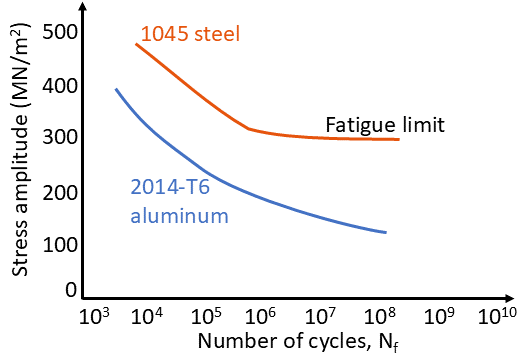
\includegraphics[angle=0, width=4in]{Material Properties-Figures/SN Curve.png}
\vspace{-2mm}
\caption{\small \blue{Taken from TAM251 Lecture Notes - L3S6}}
\vspace{-3mm}
\label{Fig:SNCurve}
\end{figure*}

\noindent If stress does not exceed the elastic limit, the specimen returns to its original configuration. However, this is not the case if the loading is repeated thousands or millions of times. In such cases, rupture will happen at stress lower than the fracture stress - this phenomenon is known as fatigue.
